
\documentclass[12pt,a4paper]{article}
\usepackage{acn-scientific}
\usepackage{acn-questions}
\usepackage[latin1]{inputenc}
\usepackage{amsmath}
\usepackage{amsfonts}
\usepackage{amssymb}
\usepackage{paracol} % for dual column
\usepackage[makeroom]{cancel}
\usetikzlibrary{decorations.pathreplacing,
  decorations.markings,
  decorations.pathmorphing}
\usetikzlibrary{arrows,shapes}

\newcommand{\quantlabel}[8][]{\node[text width=#8,fill=#6!40] (#5) at (#7) {the \emph{#2} \par #1 \par unit: \textbf{#3} (\si{#4})};}
\newcommand{\numlabel}[4]{\node[text width=#4,fill=lightgray!40] (#2) at (#3) {#1};}

\setcounter{secnumdepth}{0}
\setlength{\fboxsep}{15pt}

\title{Formulas given on IGCSE Physics Exam}
\author{\textsc{A.C. Norman}
\\ \href{mailto:ACN.Norman@radley.org.uk}{\texttt{ACN.Norman@radley.org.uk}} }
\date{}

\begin{document}

\maketitle

\tikzstyle{every picture}+=[remember picture]
%  \tikzstyle{na} = [baseline]

\columnratio{0.75}

\noindent\begin{paracol}{2}
$\text{energy transferred}=\text{current}\times\text{voltage}\times\text{time}$
\switchcolumn
$E=I\times V\times t$\\
\end{paracol}

\noindent\begin{paracol}{2}
$\text{pressure}\times\text{volume}=\text{constant}$
\switchcolumn
$p_{1}\times V_{1}=p_{2}\times V_{2}$\\
\end{paracol}

\noindent\begin{paracol}{2}
$\dfrac{\text{pressure}}{\text{temperature}}=\text{constant}$
\switchcolumn
$\dfrac{p_{1}}{T_{1}}=\dfrac{p_{2}}{T_{2}}$\\
\end{paracol}

\noindent\begin{paracol}{2}
$\text{frequency}=\dfrac{1}{\text{time period}}$
\switchcolumn
$f=\dfrac{1}{T}$\\
\end{paracol}

\vspace{0.5em}

\noindent\begin{paracol}{2}
$\text{power}=\dfrac{\text{work done}}{\text{time taken}}$
\switchcolumn
$P=\dfrac{W}{t}$\\
\end{paracol}

\vspace{0.5em}

\noindent\begin{paracol}{2}
$\text{power}=\dfrac{\text{energy transferred}}{\text{time taken}}$
\switchcolumn
$P=\dfrac{W}{t}$\\
\end{paracol}

\vspace{0.5em}

\noindent\begin{paracol}{2}
$\text{orbital speed}=\dfrac{2\pi\times\text{orbital radius}}{\text{time period}}$
\switchcolumn
$v=\dfrac{2\times\pi\times r}{T}$\\
\end{paracol}

\vspace{0.5em}

\noindent\begin{paracol}{2}
$\text{(final speed)}^{2}=\text{(initial speed)}^{2}+(2\times \text{acceleration}\times \text{distance moved})$
\switchcolumn
$v^{2}=u^{2}+(2\times a\times s)$\\
\end{paracol}

\section*{Triple}

\columnratio{0.7}

\noindent\begin{paracol}{2}
$\text{force}=\dfrac{\text{change in momentum}}{\text{time taken}}$
\switchcolumn
$F=\dfrac{(mv-mu)}{t}$\\
\end{paracol}

\vspace{0.5em}

\noindent\begin{paracol}{2}
$\text{change in thermal energy}=$\\
\hspace*{1.5cm}$\text{mass}\times\text{specific heat capacity}\times\text{change in temperature}$\\
\switchcolumn
$\Delta Q=m\times c\times\Delta T$\\
\end{paracol}

\vspace{0.5em}

\noindent\begin{paracol}{2}
$\dfrac{\text{change in wavelength}}{\text{reference wavelength}}=\dfrac{\text{velocity of a galaxy}}{\text{speed of light}}$
\switchcolumn
$\dfrac{(\lambda-\lambda_{0})}{\lambda_{0}}=\dfrac{\Delta\lambda}{\lambda_{0}}=\dfrac{v}{c}$\\
\end{paracol}


\thispagestyle{empty}

\vfill{}
\ccbyncsa
\end{document}


\framebox{
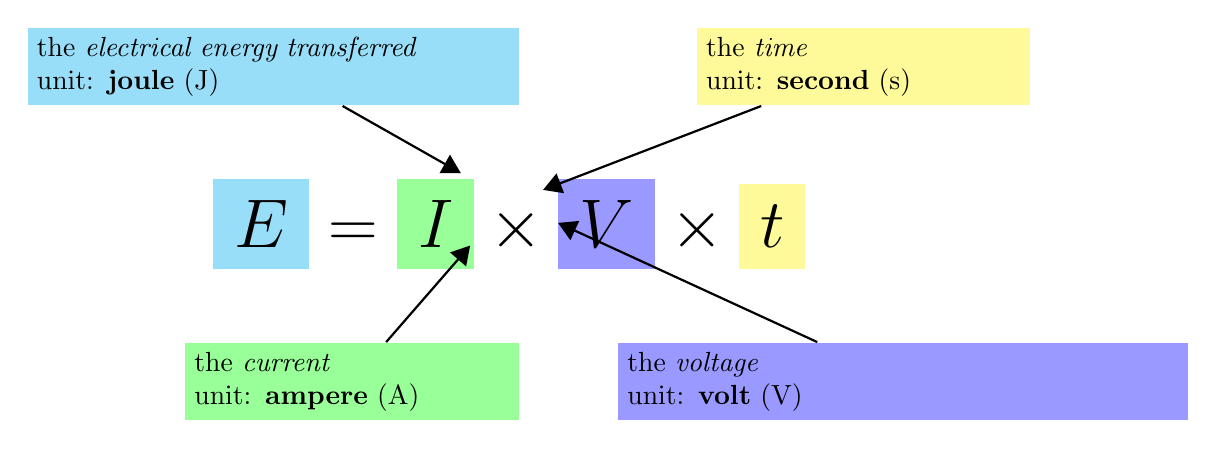
\begin{tikzpicture}[labelpointer/.style={thick, ->, >=triangle 60},]
\quantlabel{electrical energy transferred}{joule}{J}{n1}{cyan}{-3,2}{6cm}
\quantlabel{current}{ampere}{A}{n2}{green}{-2,-2}{4cm}
\quantlabel{voltage}{volt}{V}{n3}{blue}{5,-2}{7cm}
\quantlabel{time}{second}{s}{n4}{yellow}{4.5,2}{4cm}
\node at (0,0) {\Huge $
  \tikz[baseline]{
    \node[fill=cyan!40,anchor=base] (t1) 
         {$E$};
  }
    =
    \tikz[baseline]{
      \node[fill=green!40,anchor=base] (t2)
           {$I$};
    } \times
    \tikz[baseline]{
      \node[fill=blue!40,anchor=base] (t3)
           {$V$};
    } \times
    \tikz[baseline]{
      \node[fill=yellow!40,anchor=base] (t4)
           {$t$};
    }
$ };
    \draw[labelpointer] (n1) -- (t1);
    \draw[labelpointer] (n2) -- (t2);
    \draw[labelpointer] (n3) -- (t3);
    \draw[labelpointer] (n4) -- (t4);
\end{tikzpicture}
}
